\documentclass[12pt, a4paper]{article}

\usepackage[czech]{babel}
\usepackage{lmodern}
\usepackage[utf8]{inputenc}
\usepackage[T1]{fontenc}
\usepackage{graphicx}
\usepackage{listings}
\usepackage{float}
\usepackage[dvipsnames]{xcolor}

\newcommand{\img}[1]{(viz obr. \ref{#1})}

\newcommand\YAMLcolonstyle{\color{red}\footnotesize}
\newcommand\YAMLkeystyle{\color{black}\footnotesize}
\newcommand\YAMLvaluestyle{\color{blue}\footnotesize}

\makeatletter

% here is a macro expanding to the name of the language
% (handy if you decide to change it further down the road)
\newcommand\language@yaml{yaml}

\expandafter\expandafter\expandafter\lstdefinelanguage
\expandafter{\language@yaml}
{
  keywords={true,false,null,y,n},
  keywordstyle=\color{darkgray}\bfseries,
  basicstyle=\YAMLkeystyle,                                 % assuming a key comes first
  sensitive=false,
  comment=[l]{\#},
  morecomment=[s]{/*}{*/},
  commentstyle=\color{purple}\ttfamily,
  stringstyle=\YAMLvaluestyle\ttfamily,
  moredelim=[l][\color{magenta}]{*},
  moredelim=**[il][\YAMLcolonstyle{:}\YAMLvaluestyle]{:},   % switch to value style at :
  morestring=[b]',
  morestring=[b]",
  literate =    {---}{{\ProcessThreeDashes}}3
                {>}{{\textcolor{red}\textgreater}}1     
                {|}{{\textcolor{red}\textbar}}1 
                {\ -\ }{{\mdseries\ -\ }}3,
}

% switch to key style at EOL
\lst@AddToHook{EveryLine}{\ifx\lst@language\language@yaml\YAMLkeystyle\fi}
\makeatother

\newcommand\ProcessThreeDashes{\llap{\color{cyan}\mdseries-{-}-}}

\begin{document}
	\thispagestyle{empty}
	\begin{center}
		\begin{minipage}{0.75\linewidth}
		    \centering

		    \vspace{1cm}
		    
\includegraphics[width=0.75\linewidth]{fav-logo}\\
		    \vspace{2cm}

		    {\uppercase{\Large KIV/WEB \\ \textbf{Webové stránky konferenčního systému}\par}}
		    \vspace{3cm}

		    {\Large Patrik Janoušek - A17B0231P\par}
		    \vspace{2cm}

		    \vspace{1cm}

		    {\Large 6. ledna 2019}
		\end{minipage}
	\end{center}
	\pagebreak

    \tableofcontents
    \pagebreak

    \section{Instalace}
    Se zprovozněním aplikace by nikdo neměl mít žádný problém. Aplikace neklade na softwarovou výbavu systému žádné speciální požadavky.

    K běhu aplikace je pořeba webový server (např. Apache) a PHP ve verzi 7.3. Pravděpodobně bude fungovat i PHP 7.1, nicméně podpora této verze nebyla otestována.

    VirtualHost ve webovém serveru apache stačí nakonfigurovat obdobně podle následující konfigurace:
    \begin{lstlisting}
<VirtualHost *:80>
    ServerName kiv-web.localhost
    DocumentRoot "/var/www/kiv-web/public"

    <Directory "/var/www/kiv-web/public">
       Options +FollowSymLinks
	    Require all granted
	    RewriteEngine On

	    RewriteCond %{REQUEST_FILENAME} !-d
	    RewriteCond %{REQUEST_FILENAME} !-f
	    RewriteRule ^ index.php [L]
    </Directory>
</VirtualHost>
    \end{lstlisting}

    Dále je potřeba vytvořit symbolický odkaz {\tt public/storage} na {\tt storage} pomocí příkazu {\tt ln -s \$PWD/storage \$PWD/public/storage}. Aby příkaz fungoval správně, tak je nutné být v kořenovém adresáři projektu.

    Poté stačí nakonfigurovat proměnné v souboru {\tt .env}, naimportovat databázi do databázového systému MySQL (nebo některého z jeho forků). Ve výchozím stavu existuje v databázi administrátorský účet se jménem i heslem {\tt admin}.

    \section{Použité technologie}
    Aplikace byla postavena na technologiích PHP 7.3, MySQL (konkrétně MariaDB), a dodávaná konfigurace je pro webový server Apache. Neměl by však být žádný problém tuto aplikaci spustit na nginxu nebo jiném webovém serveru.

    Pro lepší správu knihoven byl použit balíčkovací nástroj composer, který se stará i o autoloading podle standardu PSR-4, kterého aplikace hojně využívá.

    Jako šablonovací systém byl použit Twig, který je vyvíjen jako jedna z komponent Symfony frameworku. Tento systém se stará o sestavení výsledného HTML dokumentu z několika různých částí. Tento šablonovací systém je také další vrstvou ochrany před XSS útoky.

    Pro sestavení JavaScript a CSS souborů je použit nástroj gulp. Tento nástroj se stará o kompilaci a minifikaci kaskádových stylů z SCSS do CSS, aby jim rozumněl prohlížeč. Stejně tak probíhá kompilace a minifikace JavaScript souborů, které jsou psány podle standardu ES6. Výstupem z tohoto nástroje je pak jeden JavaScript a jeden CSS soubor. Díky tomu je možné efektivně využít cache prohlížeče. A vzhledem k tomu, že tyto soubory nejsou nějak velké, tak to nijak negativně neovlivňuje ani první načtení webové aplikace.

    Všechny frontend knihovny jsou pak importování přes balíčkovací systém npm, který obdobně jako composer umožňuje snadnou správu a používání externích knihoven a frameworků.

    \section{Adresářové struktura}
    \begin{itemize}
    	\item app - Hlavní logika aplikace
    	\begin{itemize}
    		\item Http - Jedná se o soubory, které se nějak přímo podílí na zpracování HTTP požadavku.
    		\begin{itemize}
    			\item Controllers - Složka s controllery aplikace
     		\end{itemize}
     		\item Models - Modelová vrstva aplikace
     		\item Validators - Validátory pro jednotlivé formuláře aplikace
    	\end{itemize}
    	\item bootstrap - Skripty, které se starají o inicializační nastartování aplikace
    	\item core - Jádro aplikace. Velmi zjednodušeně řečeno se zde nachází {\it micro-framework}, který umožňuje celou aplikaci vyvíjet pohodlněji.
    	\item public - Veřejná část webu. Zde se také nachází {\tt index.php} jako jediný PHP soubor. Díky tomu není možné spouštět z veřejné části webu jiné PHP soubory než právě zmíněný {\tt index.php}, což přináší větší bezpečnost celé aplikace.
    	\begin{itemize}
    		\item dist - Zkompilované CSS a JavaScript soubory
    	\end{itemize}
    	\item resources - Složka se skripty, styly, šablonami a daty pro validátor formulářů
    	\begin{itemize}
    		\item scripts - Zdrojové JavaScript soubory před kompilací
    		\item styles - SCSS soubory
    		\item templates - Šablony pro šablonovací systém Twig
    		\item validation - Data pro validační systém. Chybové hlášky a překlady názvů jednotlivých polí.
    	\end{itemize}
    	\item routes - Jednotlivé cesty v aplikaci. Zde se nachází mapování URI adres na konkrétní metodu v konkrétním controlleru.
    	\item storage - Úložiště aplikace
    	\item .babelrc - Informace pro převedení JavaScriptu do srozumitelné podoby pro prohlížeč.
    	\item .env - Proměnné prostředí. Slouží ke konfiguraci aplikace.
    	\item .env.example - {\it Šablona} pro {\tt .env}. Pokud soubor {\tt .env} neexistuje, tak je nutné ho vytvořit jako kopii tohoto souboru. Tento soubor aplikace ignoruje.
    	\item composer.json - Konfigurace aplikace pro balíčkovací systém composer.
    	\item gulpfile.js - Postupy kompilace pro jednotlivé části aplikace pro nástroj gulp.
    	\item package.json - Konfigurace pro balíčkovací systém npm.
    	\item README.md - Návod pro instalaci aplikace
    \end{itemize}

    \section{Architektura aplikace}
    Aplikace výužívá obecně uznávaný návrhový model MVC. Díky tomu je oddělana aplikační logika, komunikace s databází a šablony pro šablonovací systém.

    \subsection{Průchod HTTP požadavku aplikací}
    Vše začíná u samotného souboru {\tt index.php}, který obsahuje pouze nezbytně nutné množství kódu. Stará se tedy o načtení autoloaderu z composeru a také souboru {\tt bootstrap/app.php}, který je v podstatě agregátorem souborů pro další průběh startu aplikace.

    V souboru {\tt bootstrap/app.php} se pak provádí definování {\it helper} funkcí, které zjednodušují používání aplikace a zkracují některé syntaktické zápisy, jelikož jsou často obalem pro vytváření objektů. Dále se provádí načtení proměnného prostředí ze souboru {\tt .env}, inicializace whoops frameworku, což je error handler framework, který se stará o hezčí a hlavně sdílnější chybové hlášky \img{whoops_framework}. Nakonec už je pak inicializováno samotné jádro aplikace, které se opět stará o inicializaci šablonovacího systému Twig, routovací knihovny Symfony Routing a vytvoření objektu aplikace, kde už začíná \uv{skutečný} život našeho HTTP požadavku. Pomocí symfony routingu se zjistí která metoda ve kterém controlleru se má zavolat, a také jeké parametry se jí mají předat. Z této metody je pak vrácen objekt {\tt Response}, {\tt View} nebo {\tt Redirect}. Na základě tohoto vráceného objektu se pak jádro aplikace rozhodna, zda prohlížeči vrátí vykreslenou HTML šablonu, holý text, JSON nebo ho přesměruje na jinou stránku.

    \begin{figure}
		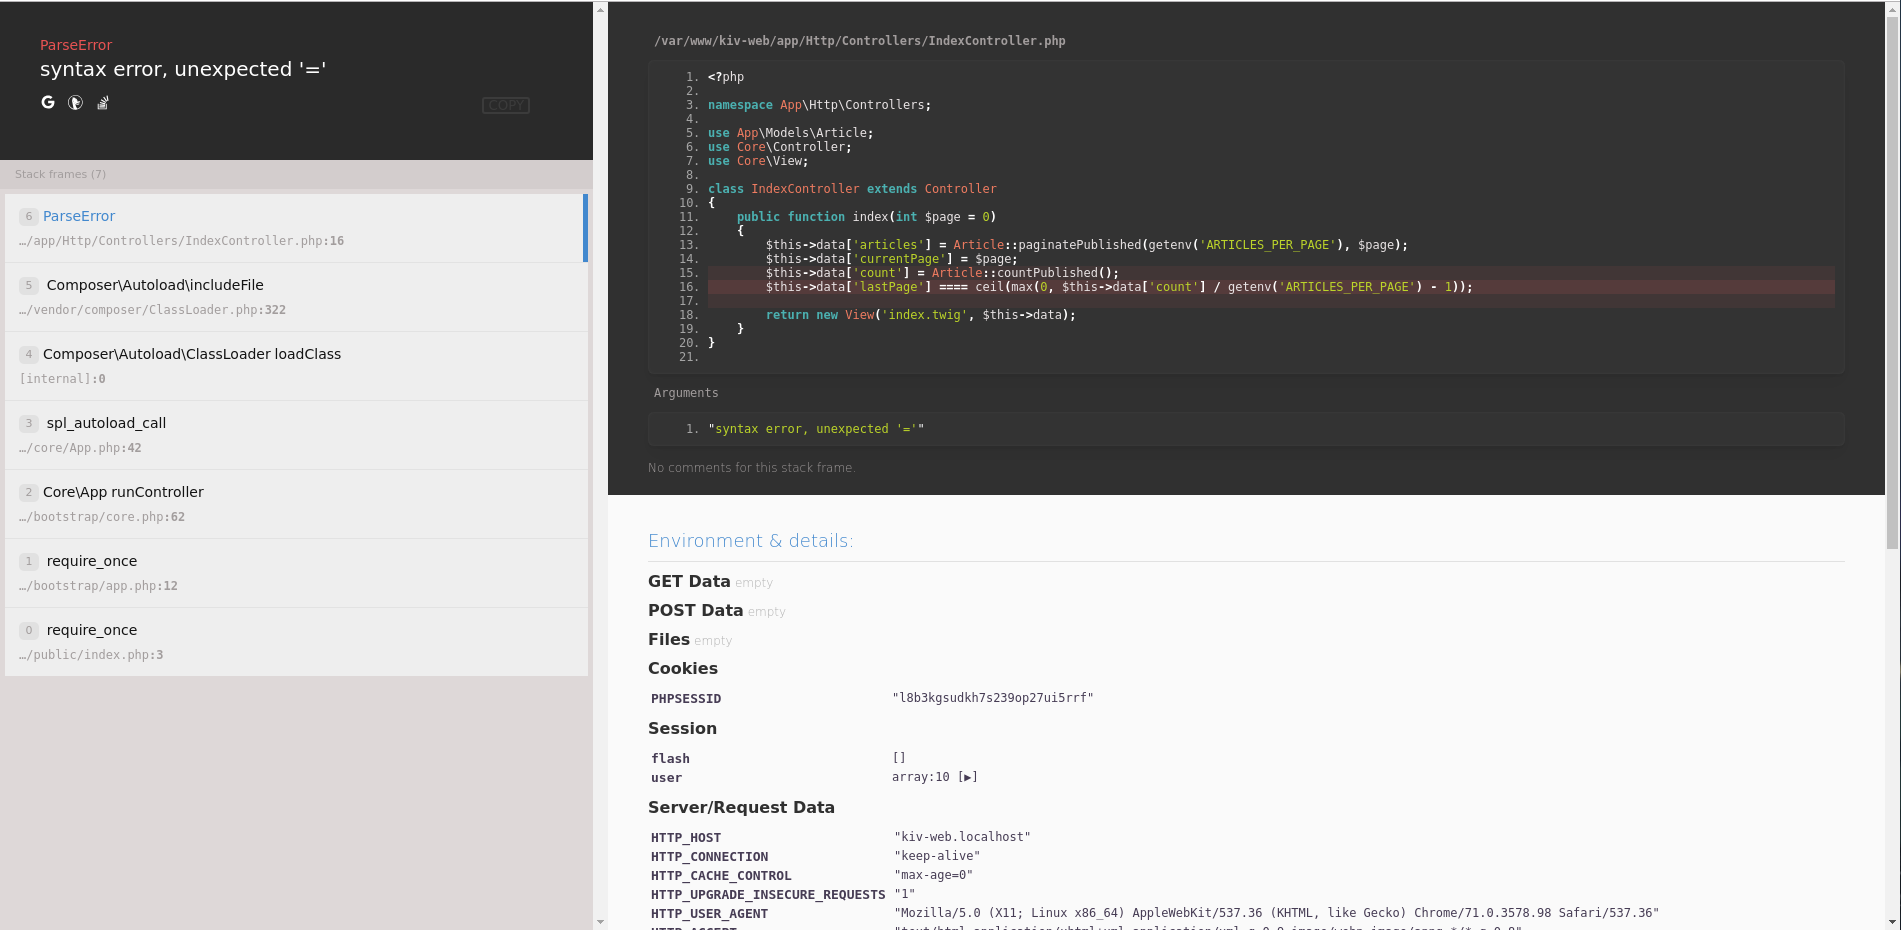
\includegraphics[width=\textwidth]{whoops_framework.png}
		\caption{Příklad chyby zobrazené Whoops frameworkem} \label{whoops_framework}
	\end{figure}

    Co se týče přesměrování, tak má aplikace podporu pro takzvané flash messages, díky kterým je možná přeposlat nějaká data mezi stránkami. To se hodí právě v případě, kdy uživatele po odeslání formuláře přesměrujeme na jinou stránku a chceme mu zobrazit nějakou informaci o tom, zda se jeho operace zdařila.

    \subsection{Definice cesty v aplikaci}
    Cesty se v aplikaci definují v souboru {\tt routes/web.yaml} ve formátu YAML, jak lze usoudit z přípony souboru. Díky tomuto je struktura velmi čistá a přehledná.

    Následující příklad ukazuje jak lze definovat cestu v aplikaci
    \begin{lstlisting}[language=yaml]
article:
    controller: App\Http\Controllers\ArticleController::showArticle
    path:
        cool:   /article/{id}
        ugly:   /?page=article&id={id}
	\end{lstlisting}

	Lze si povšimnout, že cesta má nadefinováné 2 cesty. Jsou jimi {\tt cool} a {\tt ugly}. Aplikace totiž podporuje oba styly URI a využívá se k tomu podpora Symfony Routingu pro lokalizování odkazů v aplikaci. Jedná se sice o menší zneužití této vlastnosti Symfony Routingu, ale je to jedním z nejjednodušších způsobů jak mít podporu pro oba styly URI. Přepnutí stylu URI se dá provést v {\tt .env} souboru.

	\subsection{Šablony}
	Jak již bylo zmíněno, tak šablony se nachází v adresářové struktuře nachází v {\tt resources/templates}. Tyto šablony jsou patřičně dekomponovány tak, aby bylo možné je udržitelně skládat do komplexnějších a větších šablon.

	Za zmínku stojí složka {\tt base}, ve které se nachází základní šablony pro každou část webu. Díky tomu je možné, že administrátor bude mít mírně odlišný layout než třeba autor. Soubor {\tt base.twig} je pak základním stavebním kamenem celé architektury šablon. Stanovuje obecný layout pro všechny šablony a také definuje některé klíčové proměnné pro celou aplikaci.

	\section{Uživatelské rozhraní}
	Celá webová aplikace používá velmi jednoduchý a čistý design, který je plně responzivní. Webovou aplikaci je tudíž možné používat jak z počítače, tak i tabletu nebo mobilního telefonu.

	V horní části aplikace se nachází menu, které neustále zůstává na svojí pozici. A to i tehdy, pokud se uživatel pohybuje po stránce. 

	\begin{figure}[H]
		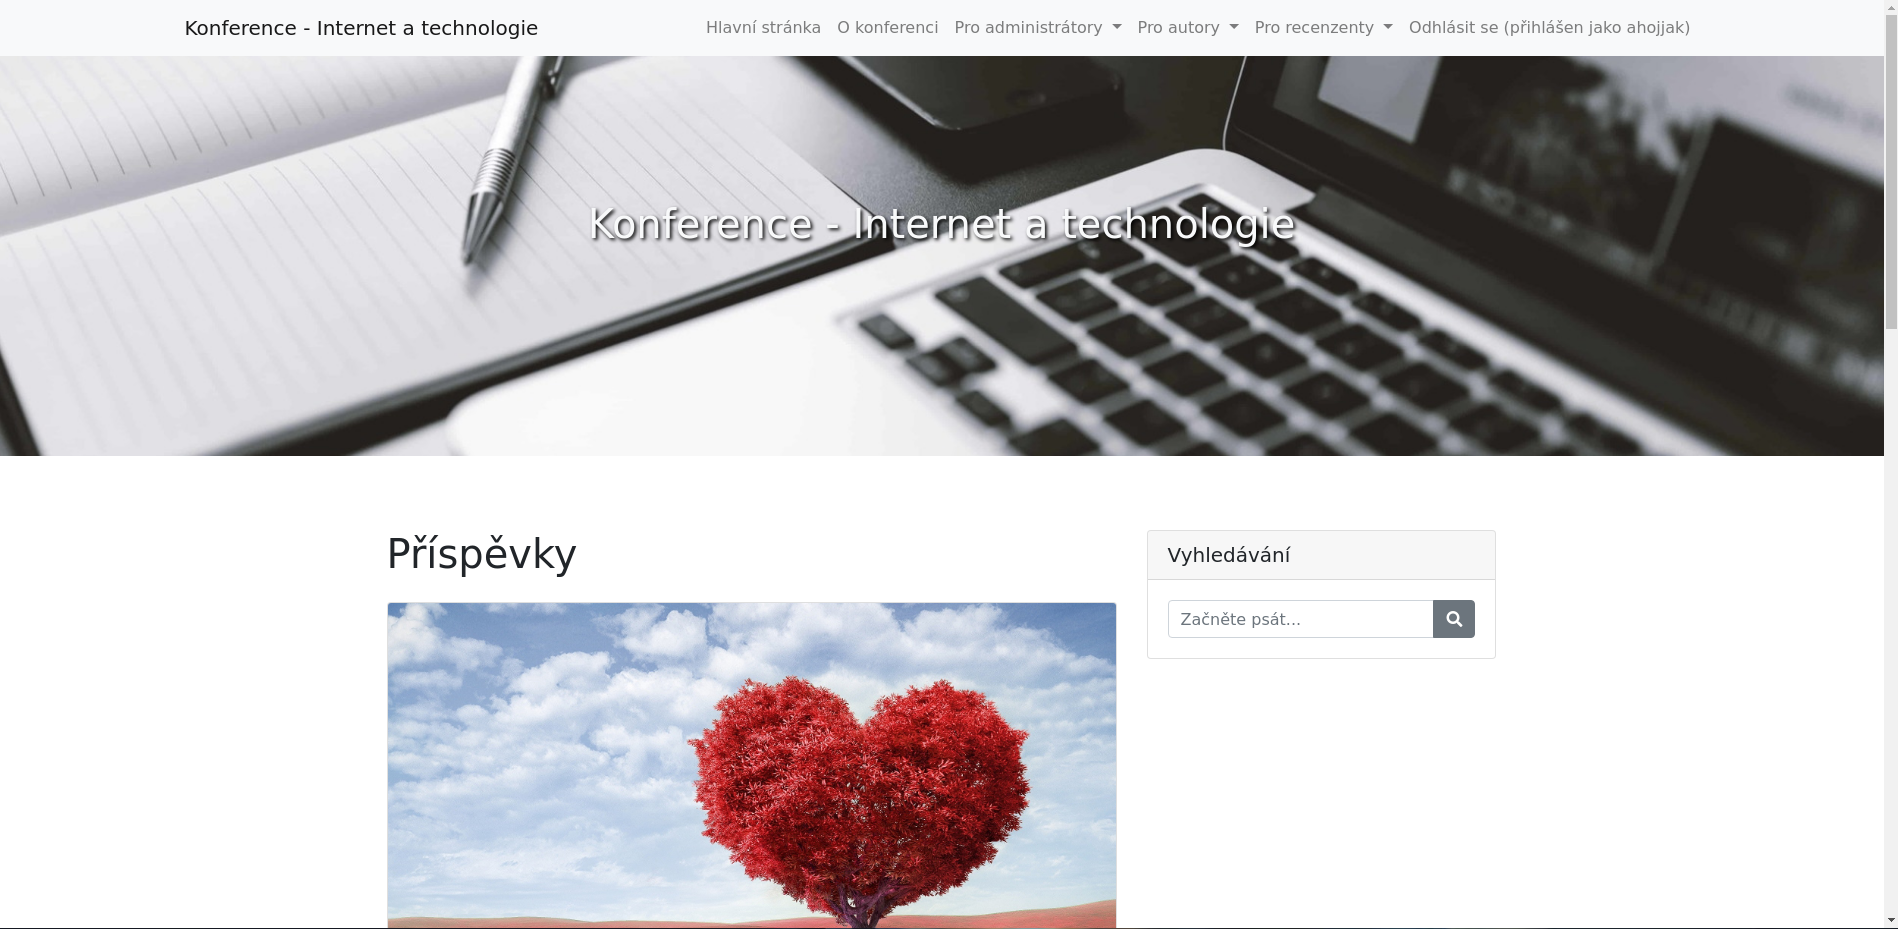
\includegraphics[width=\textwidth]{index_page.png}
		\caption{Úvodní stránka aplikace} \label{index_page}
	\end{figure}

	\section{Závěr}
	Aplikace podle mého názoru splňuje zadání v plném rozsahu. Ačkoliv jsem při vývoji nenarazil na větší překážky, tak byl velice zdlouhavý. Příčinou je pravděpodobně to, že jsem pro vypracování této semestrální práce nomohl použít PHP framework ani ORM. Díky tomu se vývoj stal mnohem pomalejším, jelikož jsem strávil spoustu hodin jenom vymýšlením rozumného jádra celé aplikace. Nicméně to určitě mělo smysl a posunulo mě to dál jako programátora. Kdybych použil například laravel, tak by to byl vzhledem k jednoduchosti aplikace jenom další web v řadě, který bych udělal za dva večery.

\end{document}
